\chapter{Theory}

To understand the strategies that follow, we first introduce three important concepts:
\begin{itemize}
\item the order of a graph $G$
\item the loose backward neighbors
\item The number of 2-coloring of a graph $G$, denoted $col_{2}(G)$
\end{itemize}

The order of a graph $G$ is a linear representation of the vertices of the graph where we associate an index to each vertex according to its position in the order.

For the loose backward neighbor, we define an order of the graph $G$: $v_{1} v_{2} v_{3}... v_{n}$. A vertex $v_{h}$ is a loose backward neighbor of $v_{i}$ if $h < i$ and if $v_{h}$ is in $v_{i}$ neighborhood, or if $v_{h}$ and $v_{i}$ have a common neighbor $v_{j}$ such as $ h < i < j$.

Now, let's review the whole range of orders for a graph $G$. For each order found, we determine the integer $k$ such as each vertex of the order has an number of loose backward neighbors $<$ to $k$. We keep the order which has the smallest $k$. This $k$ is the number of 2-coloring. In addition, the associated order satisfies $col_{2}(G)$.

\section{First strategy}

Alice determines a sequence of vertices of the graph $G$ satisfying $col_{2}(G)$. The game begins only after.

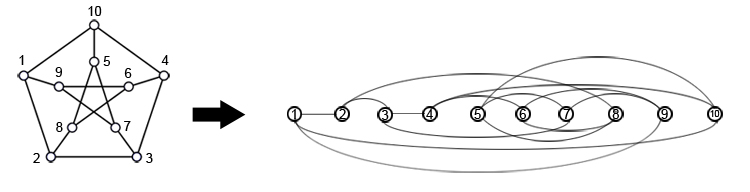
\includegraphics[width=13cm]{IntroOrder.jpg}
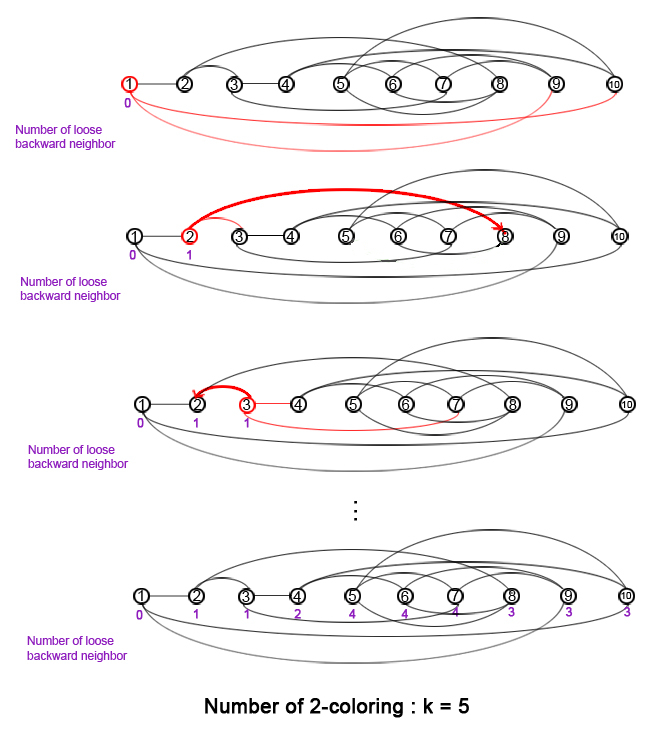
\includegraphics[width=10cm]{orderstep.jpg}

When Bob colors a vertex $v_{h}$,
Alice's strategy is to seek in the order previously determined the loose backward neigbor of $v_{h}$ not yet
colored having the lowest index. Once found, it is colored. If Alice does not find such a vertex, she simply picks from the uncolored vertices set the one with the lowest index in the order.
According to this strategy, each graph $G$ satisfies $\chi_{g}(G) \leq \chi(G) \times (1 + col_{2}(G))$.

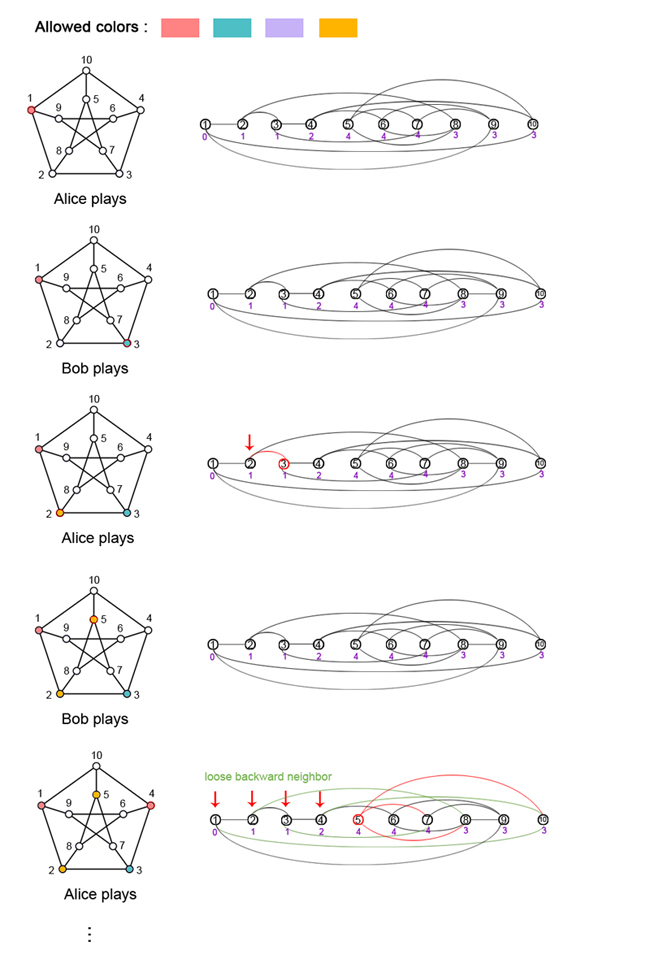
\includegraphics[width=13cm]{gameS1.jpg}
\section{Second strategy}

\section{Third strategy - Daltonism may help}

As with previous strategies, we order the vertices according to $col_{2}(G)$.
We would like to draw your attention to the fact that we no longer use the loose backward neighbors, just the backward neighbors, i.e. neighbors with a lower index in the order.

In this case, we use a rather simple activation strategy.
When Bob colors a vertex $v$, Alice begins by activating the vertex $v$, then she checks its backward neighbors.
$x$ is the backward neighbor of $v$ having the lowest index in the order.
If $x$ is colored, we turn to the next backward neighbor of $v$. If $x$ is activated, then it is in danger and we give it a color. If $x$ is not activated, then we activate it and we check its backward neighbors. If x has no unshaded backward neighbor, then we color $x$.
In the case where the vertex v (colored by Bob) has no unshaded backward neighbor, then we color the unshaded vertex having the lowest index in the order previously calculated.


According to this strategy, each graph satisfies $\chi_{g}(G) \leq 3 \times col_{2}(G) - 1$.
\section{Fourth strategy}

The purpose of this strategy is to find a better ordering of the graph $G$, on which we will use the activation strategy previously seen. We construct this order inductively (ie in the reverse order). The first selected node will be any vertex of $G$ with a degree of at most $5$.
Suppose we have already taken the vertices $v_{n}, v_{n-1}, ..., v_{i+1}$ except $v_{i}$ and we seek a candidate for $v_{i}$.

We split the vertices of $G$ into two parts: $C = (v_{n}, v_{n-1}, ..., v_{i+1})$ and $U = V \setminus C$.
We construct a new graph $H$ as follows:
\begin{itemize}
\item We remove the edges between the vertices of C.
\item We remove each vertex $v$ of $C$ having at most three adjacent vertices in $U$.
\item For each vertex $v$ removed, we add edges between its neighbors in $U$ in order to form a clique.
\end{itemize}

Now that we have our graph $H$, we assign to each edge $e$ 2 dollars spread over its vertices as follows:
\begin{itemize}
\item If $e$ connects two vertices of $U$, we give \$ 1 to each vertex of $e$.
\item If $e$ connects $x$ in $U$ and $y$ in $C$, then we give \$ 0.50 to $x$ and \$ 1.50 to $y$.
\end{itemize}

Once we have distributed the USD, we need to find a single vertex with a total value of less than \$ 6.
It will be our $v_{i}$.

When we have our order, we use the color-blind activation strategy on it.
